\chapter{Implementation}

  \vspace{-10pt}
  \section{Model Storage}

    The model was stored in a structure based off the standard half-edge data
    structure.  Each model is stored as a series of edges, vertices and faces
    that cross-reference each other.  Each face knows one edge that is a part of
    it; each vertex knows one edge that points to it and its point in space; and
    each edge knows the vertex it points to, the face it's part of, the next
    edge around the face, the previous edge around the face and the edge that
    points in the opposite direction to it along it's edge.  It is this storage
    of each real edge in two \emph{edge} structures that gives rise to the name
    half-edge.

    Along with this standard data required to completely describe a mesh in a
    half-edge structure these structs contain some additional information.  For
    performance reasons faces contain a memoized copy of their normal and edges
    contain a memoized copy of error metric result.  Obviously when an edge gets
    collapsed it will affect the normals and error metrics of the faces/edges
    around it so the two-ring of the collapsed edge has these values reset to be
    calculated again.

    An additional bit of information contained within all the structs is the
    deletion status of the face/edge/vertex, this is primarily used to simply
    determine which of the faces to draw during the display and which edges to
    consider for collapse, but is also used as a sanity check during certain
    operations to ensure deleted edges/vertices are never encountered during
    the normal processing.

  \vspace{-10pt}
  \section{Model Loading}

    The only format supported to load models from is the Object File Format
    (OFF), this is a simple list of vertices and faces composed of those
    vertices.  This means reading in the majority of the data required is very
    simple, load the vertices into an array then for each face add a series of
    edges representing the face to the edge array and the face to the face
    array.

    One limitation of the simple edge collapse algorithm used is it only
    supports triangular meshes.  This isn't much of a problem as any mesh can be
    represented as a triangular mesh, so the loading code simply complains and
    quits if any polygon with more than 3 vertices is detected.

    Once the initial set of vertices, edges and faces is loaded from file the
    rest of the data in the half-edge structure has to be calculate.  The vertex
    and face data is fully contained in the OFF format along with the edges
    previous and next pointers, the edges do however need their pair edges
    calculated.  This is done by simply iterating through the edge list and
    finding two edges (\texttt{a} and \texttt{b}) where the vertices before and
    after one (\texttt{a->vert} and \texttt{a->prev->vert}) are the same as the
    vertices after and before the other (\texttt{b->prev->vert} and
    \texttt{b->vert}) respectively.

    This takes care of the majority of the cases, however the OFF format doesn't
    contain any information about boundary edges so for those edges that don't
    have a pair found we must construct a new edge and set that as the edge,
    this pair will have its face set to \texttt{NULL} to denote that it is a
    boundary edge and will have to have both its previous and next edges (both
    also boundary edges) found.  To find these the vertices at either end of the
    new edge are rotated around (widdershins for the vertex the edge points at
    and clockwise for the other) until either another boundary edge is
    encountered or there are no more edges.  If another boundary edge is
    encountered then the two are joined as next and previous, otherwise it will
    be joined later when the missing boundary edge is added.

  \vspace{-10pt}
  \section{Error Metrics}

    Before actually calculating the error metrics a few simple tests are
    performed to weed out edges we don't care about.  First the memoized value
    of the edge is checked and returned if it is valid, after the first
    iteration this will be set for the vast majority of edges and can be easily
    returned.  Next the edge and its pair is checked if their face is
    \texttt{NUll}, if so it is a boundary edge and is skipped.  Next the one
    ring neighbourhood of both end points are checked for any boundary edges and
    if found the edge is skipped.  Some of these edges are collapsible, but
    there are a lot of special cases that aren't and others that require
    additional work to collapse so it is easier to just ignore this set of
    edges.

    Finally the intersection of the one ring neighbourhood of the end points is
    checked to ensure it only contains 2 vertices, otherwise the removal of this
    edge will cause at least four other triangles to be collapsed into lines.
    
    Both error metrics only needed two values calculable, the length
    of an edge and the angle between two face normals.  The length is trivial to
    find, it is simply the length of the vector between the points at the
    vertices of the edge, this was taken care of by the geometry library.  The
    angle between the two face normals was similarly simple to calculate by
    using the relationship $\theta = \cos^{-1}\left(m_1 \cdot m_2\right)$ where
    $m_1$ and $m_2$ are the unit normals of the two faces.  To simplify the
    calculation of this angle a mapping of $o = \frac{1 - m_1 \cdot m_2}{2}$ was
    used, this provides $o$ which follows a similar shape as $\theta$ and has
    output between 0 and 1 as seen in Fig. \ref{theta-vs-o}.

    \begin{figure}
      \centering
      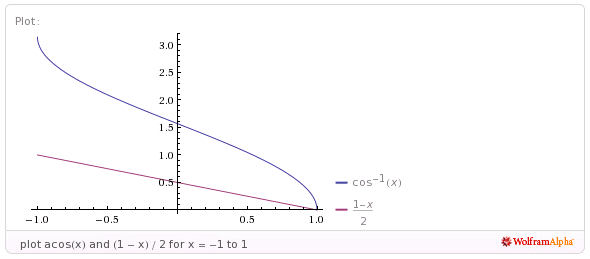
\includegraphics[width=0.5\textwidth]{images/theta-vs-o}
      \caption{$\theta$ against $o$ in the range $m_1 \cdot m_2 = [-1,1]$ \label{theta-vs-o}}
    \end{figure}

    For the simple error metric the length of the edge was simply added to the
    angle between the two faces on either side of the edge.

    For the error metric described by Stan Melax there was a bit more processing
    involved.  As stated in his paper the cost formula was:

    \begin{equation*}
      \text{cost} \left( u, v \right) =
            \left|\left|u - v\right|\right| \times
            \max_{f \in T_u} \left(
              \min_{n \in T_{uv}} \left(
                \frac{1 - m_f \cdot m_n}{2}
              \right)
            \right)
    \end{equation*}

    Where $u$ and $v$ are the end points of the edge, $T_u$ is the set of faces
    that contain $u$ and $T_{uv}$ is the set of faces that contain both $u$ and
    $v$.  In all cases that we care about $T_{uv}$ contains only two faces,
    those adjacent to the edge $\overline{uv}$.  So to calculate this we simply
    need to iterate around all edges terminating at $u$ and find the minimum of
    the angle between the normals of the corresponding face and each side of the
    $\overline{uv}$ edge.  The maximum value from this iteration is then taken
    and multiplied by the length of the edge and used as the cost.

  \vspace{-10pt}
  \section{Edge Collapse}

    \begin{figure}
      \centering
      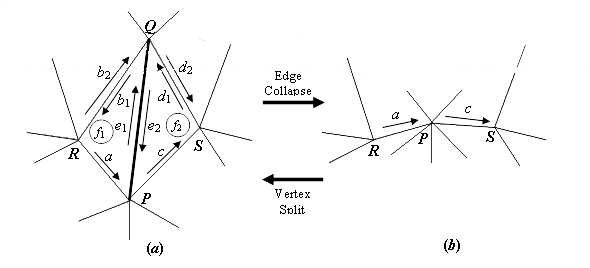
\includegraphics[width=0.5\textwidth]{images/edge_collapse}
      \caption{The edge collapse operation \label{edge_collapse}}
    \end{figure}

    Once an edge to collapse has been found the actual edge collapse must
    happen.  The identifiers used in the next section refer to those in Fig.
    \ref{edge_collapse}.

    The first operation is to connect $a$ and $c$ to the other vertices in their
    new faces, this is done by setting $a$'s previous and next to $b_2$'s
    previous and next and similarly for $c$ and $d_2$.  One special case if when
    $b_2$ and $d_2$ are part of the same triangle, in this case $a$'s next is
    set to $c$ and $c$'s prev to $a$.

    Next if $P$'s associated edge was $e_2$ then we set it to $a$ to ensure
    \texttt{p->edge} will be usable in the future.  We then traverse the edges
    of $Q$ widdershins between $d_1$ and $b_2$ and set them to point at $P$
    instead.

    We then connect the next and previous of $b_2$ and $d_2$ to point and $a$
    and $c$ respectively to finalise those triangles connections.  The faces
    associated with the triangles along with $R$ and $S$ also have their edges
    set to $a$ and $c$ to ensure they point at current edges.

    Then depending on the error metric used $P$ is either moved to the midpoint
    of the line between $P$ and $Q$ or left where it is.

    Finally the edges $e_1$, $e_2$, $b_1$, $b_2$, $d_1$, $d_2$, the faces $f_1$,
    $f_2$ and the point $Q$ all have their deleted flag set to ensure the won't
    be used in future operations.
